\chapter{Preliminaries}\label{sec:prel}

This chapter will start out by laying out some ground work for later sections.

There seems to be no ubiquitous domain language on the various cardinality analyses floating around in papers over the years, so \cref{sec:zoo} will provide a glossary for that.

We'll give abridgements of the two analyses we aim to generalise in \cref{sec:callarity} and \cref{sec:dmdanal}.

\section{Analysis Zoo}\label{sec:zoo}

Prior work disagrees in what meaning they assign to different concepts related to analyses that track evaluation counts in some way.

Just to name an example, the concept of \emph{demand} within GHC refers to a pair of strictness and usage information, while \textcite[appendix~C.2]{warnsbrough} defined demand as evaluating a binding to weak head normal form (WHNF), as opposed to applying the bound expression to one argument (\emph{use}).

\subsection{Cardinality Analysis}\label{sec:card}

A \emph{cardinality analysis} answers questions regarding how often some syntactic thing is used with respect to a single evalutation of the outer context.

Let us understand this by examining the following example:

\begin{haskellcode}
  main = do
    let a = ...
        b = ...
        c = ...
        d = ...
        e = ...
    print (a + if b then a*d else c*c)
\end{haskellcode}

A sophisticated compiler for a lazy language can find out the following facts, always assuming a single execution of \hsinl{main}:
\begin{itemize}
  \item The binding for \hsinl{a} is evaluated at least once.
  \item The binding for \hsinl{b} is evaluated exactly once.
  \item The binding for \hsinl{c} is either evaluated twice or not at all.
  \item The binding for \hsinl{d} is either evaluated once or not at all.
  \item The binding for \hsinl{e} is absent, \eg not used even once.
\end{itemize}

Based on these facts, the compiler can apply a number of optimisations:
\begin{description}
  \item[Call-by-value] 
    Since \hsinl{a} and \hsinl{b} are evaluated \emph{at least once}, the compiler is free to apply a call-by-value evaluation strategy for them.
    Recovering strictness in this way makes a huge difference, as subsequent transformations such as a worker/wrapper transformation \parencite{ww} may exploit this information to great effect.
  \item[Call-by-name]
    Because \hsinl{b} and \hsinl{d} are evaluated \emph{at most once}, the compiler can employ a call-by-name strategy instead of call-by-need.
    Operationally, this omits unnecessary thunk updates for these so-called \emph{single-entry} thunks, because the computed value doesn't need to be memoised.
  \item[Absence]
    The example doesn't mention any use of \hsinl{e}. 
    Such absence can be exploited by not generating code for the binding at all, or replace the binding by an error message in case of analysis failure.
    Absence is also important for the worker/wrapper transformation \parencite{ww}, in that it conjures custom calling conventions that won't need to mention (partially) absent arguments at all.
\end{description}

Of course, call-by-value and call-by-name are mutually exclusive, which means that for \hsinl{b} the compiler must choose between the two. 
In practice, that is an easy choice: 
Call-by-value enables much more effective optimisations than call-by-name.
Nonetheless, the share of single-entry thunks is dominating (70\% according to same dated results of \textcite{updabs}) and deemed worth optimising.

Note that we only care for the three cardinalities $\{0, 1, \omega\}$ in our examples:
Everything beyond the second evaluation carries no usable information, thus we denote the cases of `evaluated multiple times' with $\omega$.

As in the above example, possible cardinality may also depend on runtime information, so that information is better reflected as a subset of $\{0, 1, \omega\}$.
Most interesting, however, are the over-approximating (\eg maximum) and under-approximating (\eg minimum) cardinalities, which act as proofs for the compiler to justify said optimisations.

Thus, a cardinality analysis assigns each binding an interval of its maximum und minimum evaluation cardinality, relative to a single evaluation of the binding site.

In the example above, \hsinl{a} would be annotated with $[1,\omega]$ (evaluated at least once, possibly many times), whereas the absent \hsinl{e} would be annotated with $[0, 0]$ (evaluated at most never).

This is exactly the notion of usage-interval analysis in \textcite[chapter~5]{sestoft}, which defines `usage count' as what we call cardinality.
As observed by \parencite[section~1.5]{warnsbrough}, this corresponds to the Bierman lattice \parencite{bierman} without the $\neq 1$ case.

\subsection{Strictness Analysis}\label{sec:strict}

Analogous to the distinction of alias analyses between \MayAlias and \MustAlias in typical imperative languages, cardinality analysis can be split in two separate passes:
\MinCard and \MaxCard. Looking at the \MinCard problem, the only information that is exploited by compilers so far is that of \emph{strictness}.

An expression \hsinl{... let x = e in body ...} is strict in the binding \hsinl{x} if the whole expression diverges whenever \hsinl{e} does.
Put another way: 
If an expression is \emph{strict} in some binding \hsinl{x}, the expression will certainly evaluate \hsinl{x} on all code paths, \eg \hsinl{x} is evaluated at least once.

Finding out whether or not a binding is evaluated at least once, relative to a single evaluation of the binding expression, is the goal of \emph{strictness analysis}.
Strictness analysis enables the call-by-value optimisations explained above and caters for the worker/wrapper transformation \parencite{ww}.

Note that from a \MinCard perspective, there is at least one more bit of information that would also be of interest, namely if a binding is evaluated \emph{at least multiple times} (\eg annotation $[\omega,\omega]$).
There is no real gain for compilers in knowing that information!
This leads to delightful simplicity in the implementation of strictness analysis compared to \MinCard or \MaxCard in the case of thunks.

\todo{Pick this up in a later section}

\subsection{Usage Analysis}\label{sec:usage}

Strictness analysis captures all necessary information on \MinCard, \eg if $\alpha$ in the annotation $[\alpha,\beta]$ is $0$ or $1$.

We refer to the analogue of \MaxCard as a \emph{usage analysis}.
A usage analysis provides an over-estimate to cardinality.
For a given binding, it finds out \emph{at most} how often the binding is evaluated in a single evaluation of the binding expression.

Both \emph{absence analysis} (\eg, is $\beta$ in the cardinality annotation $[\alpha, \beta]$ at most 0?) and \emph{sharing analysis} (\eg, is $\beta$ in the cardinality annotation $[\alpha, \beta]$ at most 1?) are generalised by usage analysis.

The results of a sharing analysis support the call-by-name optimisation from above, while absence information is needed together with strictness information for the worker/wrapper transform.

As \textcite[section~2.4]{verstoep} points out, a sharing analysis finds out similar results as a \emph{uniqueness analysis}.
They serve different purposes, however; Uniqueness information is propagated during type-checking and may affect which programs are rejected, while sharing analysis is an enabling analysis for other optimisations in the middleend.

That also means that the benefits of uniqueness types might carry over to thunks that a sharing analysis finds to be single-entry, just by changing their type after it passed type-checking.

Less far-fetched is the benefit of identifying \emph{one-shot} lambdas.
Roughly speaking, a lambda is one-shot if a single evaluation of the expression that reduces to the lambda leads to at most one call of the lambda.

This is best understood by an

\begin{example}
  Consider the function \hsinl{f} in the following expression:
  \begin{haskellcode}
    let f x y = m*x + y
    in f 1 2 + f 3 4
  \end{haskellcode}

  The outer lambda, binding \hsinl{x}, is not one-shot:
  As the work of evaluating the expression bound to \hsinl{f} to WHNF (which it trivially has) is shared between the two calls to the lambda.

  It is different for the inner lambda, binding \hsinl{y}, however.
  In each of the two calls, the result of applying \hsinl{f} to one argument is immediately applied to another argument. The redexes $f 1$ and $f 2$ represent the relative evaluations here and in each the case the resulting lambda is called once.
  
  Thus, the lambda which binds \hsinl{y} is one-shot.
\end{example}

Recognising one-shot lambdas opens up opportunities for a number of further optimisations \parencite[section~6.6.2]{warnsbrough}:
\begin{description}
  \item[Floating]
    Normally, floating a \hsinl{let} binding inside a lambda risks duplicating shared work.
    One-shot lambdas guarantee that the body will not be evaluated more often than the containing expression, so floating bindings inside is safe.

    Note that in the above example, \hsinl{m} could not be floated inside the body of \hsinl{f}.
    Although the inner lambda (\hsinl{y}) is one-shot, the outer isn't.
  \item[$\eta$-expansion]
    Instead of floating \hsinl{let} bindings (and other syntactic things) inside a one-shot lambda, we can go the other way and float inner one-shot lambdas \emph{out}.
    This process is called $\eta$-expansion, as opposed to $\eta$-reduction.
    $\eta$-expansion is not generally safe for ordinary lambdas for the same reasons as floating \hsinl{let} bindings in, \eg duplicating work.

    $\eta$-expansion based on usage information is the key idea behind the efforts of \textcite{callarity} of making \hsinl{foldl} a good consumer for list fusion.
  \item[Inlining]
    Inlining bindings under a lambda risks duplication of shared work, which is why the inliner needs additional confirmation that the chain of lambdas under which to inline is one-shot.
    There is large overlap with the float in case, but remember that inlining may be beneficial in cases where a binding cannot be floated in.
\end{description}

All these opportunities boil down to the compiler being cautious not to duplicate work when shoving something under a lambda.
It seems reasonable to annotate one-shot lambdas while performing usage analysis as the information falls off as a byproduct anyway.

\section{Call Arity}\label{sec:callarity}

Call Arity \parencite{callarity} is a carefully crafted analysis with the single goal of making \hsinl{foldl} take part in list fusion without compromising in terms of allocations.

It does so by $\eta$-expanding bindings based on usage information.
This is best demonstrated by an example:
\begin{haskellcode}
  let f x = 
        if expensive
        then id 
        else (*2)
  in f 1 2 + f 4 5
\end{haskellcode}

Call Arity recognises \hsinl{f} as always being called with two arguments and justifies $\eta$-expansion of the expression bound to \hsinl{f} to arity two.
The justification for why this doesn't lose shared work of evaluating the arbitrariliy \hsinl{expensive} expression (\cf \cref{sec:usage}) is that there is no call with arity less than two, so that the sharing would never be observed.

This would be all there is to arity expansion (\eg $\eta$-expansion of the bound expression) based on usage, if it weren't for thunks:
\begin{haskellcode}
  let f =
        if expensive
        then \x y -> y
        else \x y -> y*2
  in f 1 2 + f 4 5
\end{haskellcode}

This computes the same expression as the previous example, but has different operational behavior.
Since \hsinl{f} is now a thunk (\eg binds an expression that is not in WHNF), expanding \hsinl{f} to call arity (minimum arity of each call), which is two, duplicates the work associated with evaluating \hsinl{expensive}, which would otherwise be shared between the two calls.

It is safe to $\eta$-expand thunks to call arity if they are just called once, though:
\begin{haskellcode}
  let f =
        if expensive
        then \x y -> y
        else \x y -> y*2
  in f 1 2
\end{haskellcode}

Thus, Call Arity tracks for each binder whether it was just called once and the minimum arity of each call (call arity).
The `called once' part is tracked by a sharing analysis, while call arity is just computed by a simple arity analysis.

As the examples demonstrate, the arity analysis leans on the sharing analysis.
The next example shows that information also flows in the reverse direction:
\begin{haskellcode}
  let f x = expensive
  in f 1
\end{haskellcode}

A (rather simple) sharing analysis would analyse the binding of \hsinl{f} and would have to assume that \hsinl{expensive} is evaluated possibly multiple times, because it is hidden under a lambda.
Under the assumption that \hsinl{f} is only called once, with one argument (!), the sharing analysis can conclude that \hsinl{expensive} is only used once.

Thus, the interleaving of sharing and arity analysis within Call Arity makes sense, although as we see later in \cref{sec:generalise}, call arity is just the result of exploiting one-shot and single-entry information.\smallskip

In order for Call Arity to have available the minimum call arity of an identifier when analysing its bound expression, it has to analyse \hsinl{let} from the bottom up, \eg analyse the body before the bound expression.

This is has limitations in cases like this:
\begin{haskellcode}
  let x = ...
  in let y = 2*x
     in if b
        then x
        else y
\end{haskellcode}

Here, the bottom-up sharing analysis will not find out that \hsinl{x} is only evaluated once. 
At the point where \hsinl{y} is analysed, it is already clear that \hsinl{x} was evaluated, and because \hsinl{y} was also evaluated, it seems that \hsinl{x} was evaluated twice.
That is too conservative, however: The bottom-up scheme forgot that \hsinl{y} and \hsinl{x} were evaluated on different code paths.

Thus, Call Arity employs a novel sharing analysis based on \emph{co-call graphs} instead.
Co-call graphs track which identifiers are possibly evaluated with each other by an edge.
The absence of a co-call edge proves that the unrelated identifiers are never evaluated on the same code path.

For the \hsinl{if} expression in the above example, the co-call graph looks like this:
\[  
  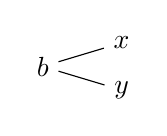
\begin{tikzpicture}[baseline={(0.base)}]
    \node (0) {$b$};
    \node at (1,0.3) (1) {$x$};
    \node at (1,-0.3) (2) {$y$};
    \draw (0) -- (1);
    \draw (0) -- (2);
  \end{tikzpicture}
\]

It properly reflects that \hsinl{x} is never called together with \hsinl{y}.
The analysis then makes use of that information when handling the \hsinl{let} expression binding \hsinl{y}, by effectively performing substitution of the co-call graph of its bound expression (which contains the single node \hsinl{x} without any edges) for \hsinl{y} in the above co-call graph of the body.

After this substitution step, there will be no loop on \hsinl{x}, because there was no edge between \hsinl{y} and \hsinl{x}.
This represents the fact that \hsinl{x} is not called with itself, or only called once, plainly speaking.

Co-call graphs and this rather involved substitution procedure are illuminated in detail in \cref{sec:graph} and \cref{sec:let}.
\Cref{sec:bench} discusses the impact of co-call graphs on analysis precision and performance.

\section{Demand Analyser}\label{sec:dmd}

Blub
